% Chapter 2

\chapter{Experimental technique} % Main chapter title

\label{Chapter2} % For referencing the chapter elsewhere, use \ref{Chapter2} 

The E989 Fermilab muon g-2 experiment, aims to measure the anomalous magnetic moment of the muon, a$_{\mu}$, to a world’s best precision of 140 ppb \cite{Reference13}. This would be an improvement of almost a factor of four compared to the current world's best precision of 540 ppb from the E821 g-2 experiment at BNL.

The experiment applies the same measurement principle as the BNL E821 experiment and uses a storage ring method to determine a value of $a_{\mu}$. In the experiment, two frequencies are measured: $\omega_a$ and $\omega_p$. $\omega_a$ is the difference between the rate the muon polarization rotates and the rate the muon momentum rotates (the cyclotron frequency) and is determined from the arrival time spectrum of the decay positrons. Along with the magnetic field normalized to the Larmor frequency of a free proton $\omega_{p}$ determined by averaging the magnetic field maps over the muon beam distribution \cite{Reference23}. This section will describe the techniques used to make this $a_{\mu}$ measurement. 

To achieve the target precision the systematic uncertainty limit on both the experimental measurements of the anomalous precession frequency $\omega_{a}$ and the magnetic field normalized to the proton Larmor frequency $\omega_{p}$ must be 70 ppb each. This would be a threefold and twofold improvement, respectively, compared to E821. Table 3.1 outlines how the precision will be improved from the E981 experiment. To achieve the goal 100 ppb statistical uncertainty, at least $1.5\times{10^{11}}$ events are needed, which is 20 times the statistics of the BNL E821 experiment.  

\begin{table}[h!]
\begin{center}
 \begin{tabular}{||c | c | m{5cm} | c||} 
 \hline
 Category & E821 [ppb] & E989 planned improvements & Goal [ppb]\\ [0.5ex] 
 \hline\hline
 Gain changes & 120 & Better laser calibration. Low energy threshold & 20\\ 
 \hline
 Pileup & 80 & Low energy samples recorded. Calorimeter segmentation & 40 \\
 \hline
 Lost muons & 90 & Better collimation in ring & 20 \\
 \hline
 CBO & 70 & Higher n value (frequency). Better match of beamline to ring & < 30 \\
 \hline
 E and pitch & 50 & Improved tracker. Precise storage ring simulations & 30 \\ 
 \hline
 Total & 180 & Quadrature sum & 70  \\ [1ex] 
 \hline
\end{tabular}
\caption{Table of the largest systematic uncertainties for the BNL E821 experiment along with the proposed upgrade plans and the improved uncertainties these plans should achieve\cite{Reference29}.}
\label{table:1}
\end{center}
\end{table}

\section{Muon precession frequencies}

The measurement of magnetic dipole moment utilises the fact that a charged particle with a non-zero magnetic moment experiences a torque in an external magnetic field. This leads to a precession of the particles spin vector about the magnetic field direction called the spin precession $\omega_{s}$. The non-relativistic equation is given by

\begin{equation}
\omega_{s} = g\frac{eB}{2m},
\end{equation}
where $g$ is the gyromagnetic ratio, $e$ the electron charge, $B$ the magnetic field and $m$ the mass of the particle.

The magnetic moment is related to the spin precession frequency as shown in equation 2.1. However as the spin precession is not an experimentally observable value, the g-factor cannot be calculated directly from $\omega_{s}$. Instead the observable measured is the precession of the average direction the decay positrons are emitted from the muons. From this $\omega_{a}$ can be determined.

A charged particle passing through a magnetic field will also undergo cyclotron motion. So a charged particle travelling through a constant magnetic field will move in a circular path with a constant radius. The non-relativistic cyclotron frequency, $\omega_{c}$ is given by
\begin{equation}
\omega_{c} = \frac{eB}{{m}}.
\end{equation}

Therefore a charged particle traversing through a constant magnetic field has a momentum vector which rotates at the cyclotron frequency $\omega_{c}$ and a spin vector which rotates at the spin frequency $\omega_{s}$. This will be discussed in more detail in section 3.4.

\section{Pion and muon decay}

Muons are produced in the parity violating weak decays of pions. The dominant pion and muon decays are shown in figure 3.1. The dominant decay of the pion is given by

\begin{equation}
{\pi^{+}}\rightarrow{\mu^{+}}\nu{_\mu}.
\end{equation}
\noindent
The implication being that the weak force only couples to left-handed particles and right-handed anti-particles. Neutrinos are left handed and as such are emitted with their spin vector antiparallel to their momentum vector. Whereas anti-neutrinos are right handed so have their spin vector parallel to their momentum vector. A pion has a spin value of zero therefore to conserve angular momentum the muon must be emitted left handed with its spin and momentum directions antiparallel. A diagram of the parity violating pion decay is shown in figure 3.2.

This can be exploited to produce a polarized muon beam. High energy polarised muons can be created by choosing forward or backward decays. Where forward or backward refers to whether the decay is forward or backward in the center-of-mass frame relative to the pion momentum. Forward decays have muons produced mostly parallel to the pion laboratory momentum. In these decays muons have the highest laboratory momentum with their polarisation opposite to the laboratory momentum. Whereas backward decays have muons produced mostly anti-parallel to the pion laboratory momentum. With these decays muons have the lowest laboratory momentum with their polarisation parallel the laboratory momentum. The g-2 experiment uses forward muon decays from a beam of polarised pions and so selects the highest energy muons produced \cite{Reference29}.

The dominant decay of the muon is also a parity violating weak interaction given by

\begin{equation}
{\mu^{+}}\rightarrow{e^{+}}\bar{\nu}{_\mu}\nu{_e}.
\end{equation}

\begin{figure}[th]
\centering
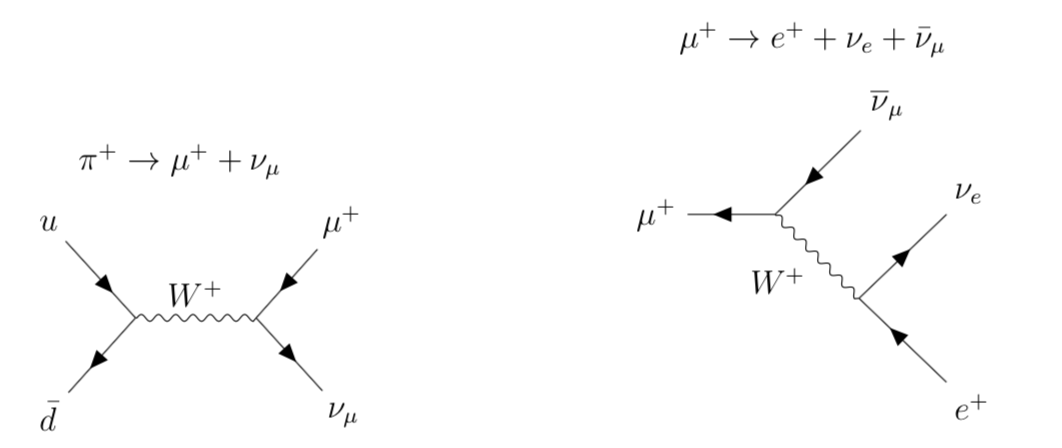
\includegraphics[scale=0.8]{Figures/muonpiondecay}
\decoRule
\caption{Feynman diagrams of the dominant decays of the pion and muon.}
\label{fig:muonpiondecay}
\end{figure}

In muon decay, the highest energy positrons have a maximum allowed energy in the muon reference frame (MRF) of $E_{max}=\frac{m_{\mu}c^2}{2}=53MeV$. In these decays the muon anti neutrino will be left handed and the electron neutrino right handed. A diagram of the parity violating muon decay is shown in figure 3.3. This means that both their momentum vectors will be parallel to each other but anti-parallel to the positron direction. As the neutrino pair contains zero total angular momentum, the decay positron will possess the muons angular momentum. In order to conserve angular momentum the positrons spin vector must be aligned with the muons spin vector. As an anti-particle the positron is right handed which implies that its spin and momentum vectors are parallel. And so in general muon decays will produce positrons that are preferentially emitted in the same direction as the muon spin. Similarly the highest energy positrons are emitted parallel to the muon spin in the MRF, with the spin of the positron directed parallel to the muons spin. Because the direction of the muon spin vector can be determined from its emission direction, the measurement of the precession of the average direction of the highest energy positrons is used to determine $\omega_{s}$.

\begin{figure}[th]
\centering
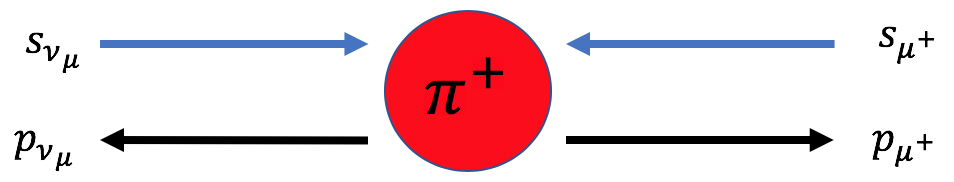
\includegraphics[scale=0.8]{Figures/piondecay.png}
\decoRule
\caption{A diagram of the parity violating pion decay.}
\label{fig:piondecay}
\end{figure}

\begin{figure}[th]
\centering
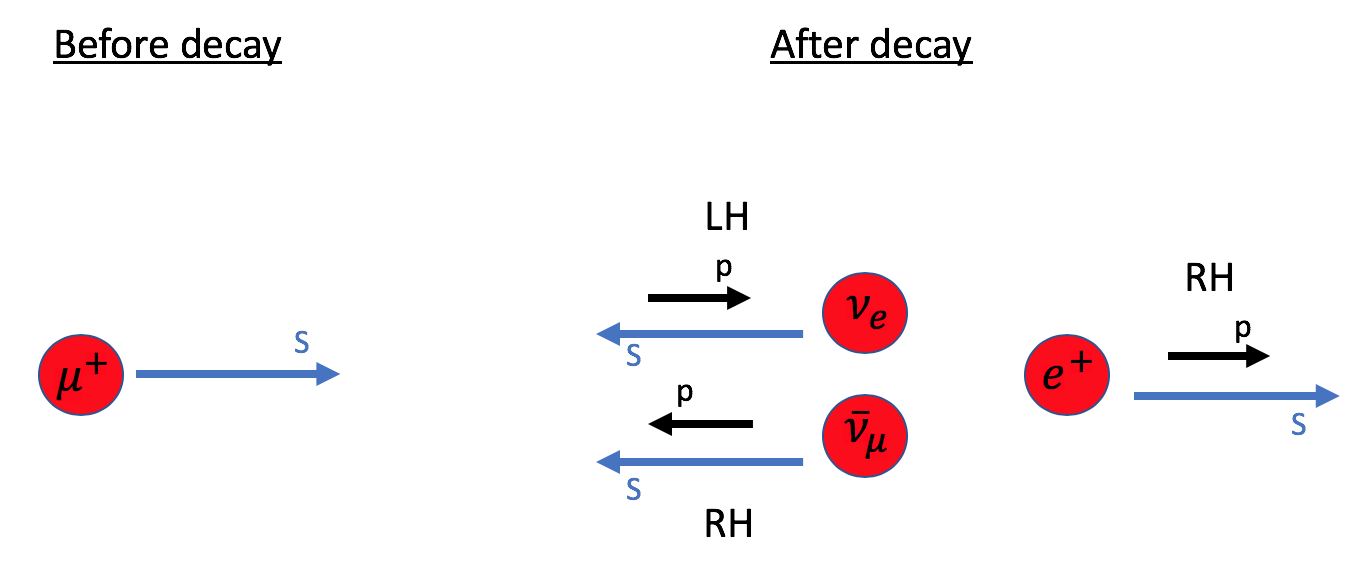
\includegraphics[scale=0.6]{Figures/muondecay.png}
\decoRule
\caption{A diagram of the parity violating muon decay.}
\label{fig:muondecay}
\end{figure}

\section{Measuring $\omega_{a}$}

The experiment will count the number of decay positrons observed above some energy threshold as a function of time. The observed oscillation gives the $\omega_{a}$ value because, as was shown earlier, decay positrons from muons with the highest energy are more likely to have their momentum direction parallel to the muons spin. Consequently choosing decay positrons above some energy threshold will lead to a measurement of the $\omega_{a}$ oscillation \cite{Reference29}.

It must be noted that if all energies of decay positrons are included in the $\omega_{a}$ calculation, the measurement of the number of positrons detected as a function of time would give an exponential decay. Therefore a cut must be made on the detected positrons to enable only the decay positrons that will lead to an $\omega_{a}$ oscillation being observed. Selecting positrons above a selected energy threshold in the laboratory frame will give positrons with a net momentum (in the MRF) parallel to the muon momentum direction. To gain the maximum $\omega_{a}$ oscillation signal possible while not having too high an energy cut which would lower the statistics available, an optimal energy cut must be chosen \cite{Reference1}\cite{Reference13}.

In the MRF the differential probability for the positron with normalised energy $y=\frac{E}{E_{max}}$ where $E_{max}=53MeV$ to be emitted at an angle $\theta$ with respect to the muon spin is given by

\begin{equation}
dP = \bigg(\frac{1}{2\pi}\bigg)N(y)[1-A(y)cos\theta]dyd\omega,
\end{equation}
\noindent
where the relative number distribution N(y) is given by
\begin{equation}
N(y)=y^2(3-2y),
\end{equation}
\noindent
and the decay asymmetry distribution is given by
\begin{equation}
A(y)=\frac{q}{e}\frac{2y-1}{3-2y}.
\end{equation}
\noindent
The asymmetry and number distributions are at maximum value when y=1 and the asymmetry distribution changes sign at a value of $\frac{1}{2}$.

\begin{figure}[th]
\centering
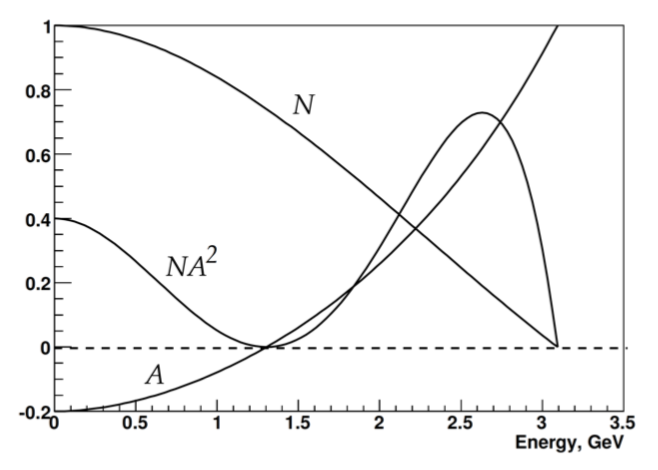
\includegraphics[scale=0.9]{Figures/NA2}
\decoRule
\caption{The relative and asymmetry distributions as a function of positron energy.}
\label{fig:NA2}
\end{figure}

The number of decay positrons above an energy threshold E with a time t after injection of muons into the storage ring, is given by

\begin{equation}
N(t)= N_0(E)e^{(-t/{\gamma}\tau_\mu)}[1+A(E)cos(\omega_{a}t+\phi(E))].
\end{equation}
\noindent
where $N_{0}(E)$ is a normalisation factor, $\tau_\mu$ the muon rest frame lifetime, and A(E) the asymmetry distribution of positrons with energy greater than the energy threshold E. 

The fractional statistical error on $\omega_{a}$, when fitting data measured over numerous muon lifetimes to equation 3.8 is given by

\begin{equation}
\sigma_{\epsilon} = \frac{\sigma_{\omega_{a}}}{\omega_{a}} = \frac{\sqrt{2}}{2\pi{f_{a}\tau_{\mu}}\sqrt{NA^2}}.
\end{equation}

The value of the differential quantity $NA^2$ shows the relative 
weight by electron energy to the ensemble average figure of merit, with equation 3.9 showing that the statistical uncertainty of a measurement of $\omega_{a}$ is inversely proportional to $NA^2$. This means that $NA^2$ needs to be maximized to minimize the statistical uncertainty on $\omega_{a}$\cite{Reference1}\cite{Reference29}.

Figure 3.4 displays the relative number and asymmetry distribution versus energy in the laboratory frame. This shows that the statistical power is greatest for a maximum value of $NA^2$ which is at 2.6 GeV. When applying a fit to all positrons above a certain energy cut, the optimal threshold energy is found to be approximately 1.8 GeV. A value for $\omega_{a}$ can then be calculated using a five parameter fit using equation 3.8. The number of positron hits as a function of time with energy greater than 1.8 GeV measured by the calorimeters for the BNL E821 experiments 2001 data set is shown in figure 3.5. This shows the g-2 oscillation in the muon exponential decay curve and how $\omega_{a}$ can be determined from this data using a fit given by equation 3.8. 

\begin{figure}[th]
\centering
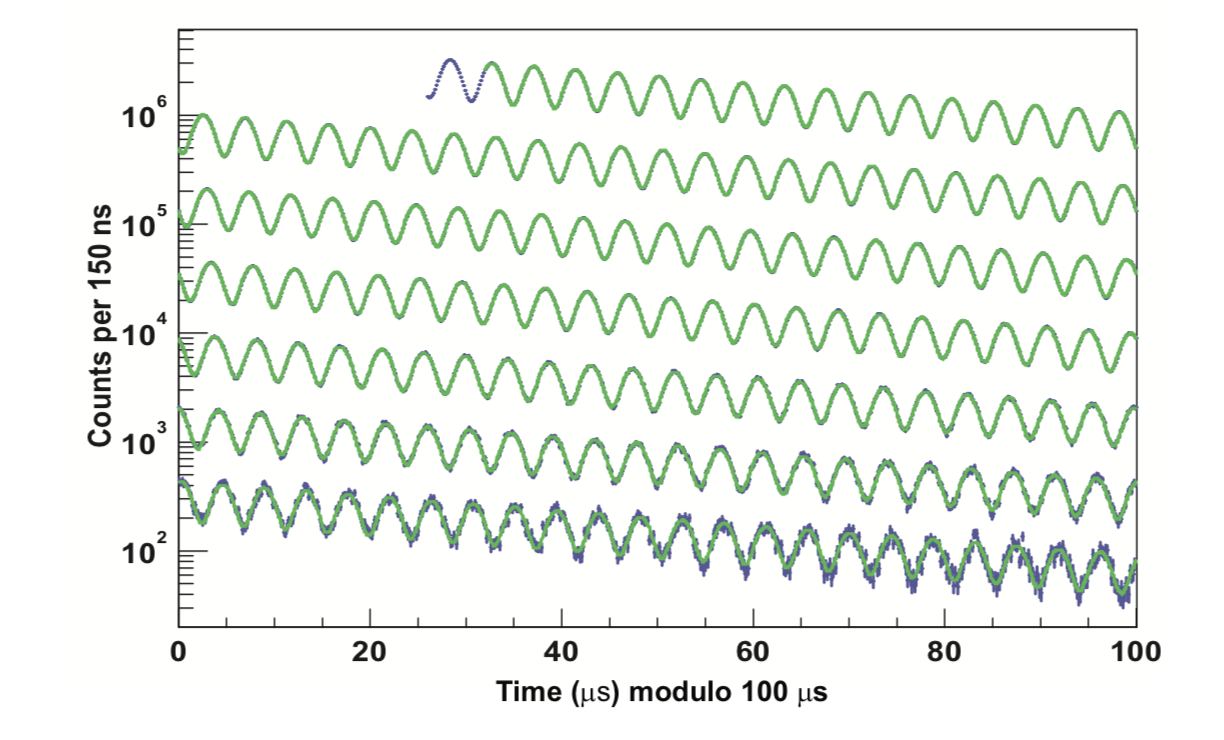
\includegraphics[scale=0.65]{Figures/wiggle}
\decoRule
\caption{Distribution of the decay positrons as a function of time with energy above 1.8 GeV for the BNL 2001 data set. Here a total of $3.6\times10^9$ positrons were used to obtain a fit to determine a value of $\omega_{a}$.}
\label{fig:wiggle}
\end{figure}

\section{$\omega_{a}$ calculation}

The muon anomaly frequency $omega_{a}$ is the frequency the spin vector precesses relative to the momentum vector. This is calculated using the difference between these two precession frequencies. A visualisation of the two frequencies is shown in figure 3.6. When the spin precession frequency is greater than the cyclotron frequency the g-factor value does not equal 2, this leads to a difference between these two frequencies. On the other hand if the muon had g = 2, then $a_{\mu}$ = 0 and so the spin and cyclotron frequencies would be equal.
The difference between these two frequencies $\omega_{a}$ = $\omega_{s}$ - $\omega_{c}$ is referred to as the anomalous precession frequency. 
\begin{equation}
\omega_{a} = \omega_{s} - \omega_{c} = \bigg(\frac{g}{2}-1\bigg)\frac{eB}{m} = a_{\mu}\frac{eB}{m}.
\end{equation}

\begin{figure}[th]
\centering
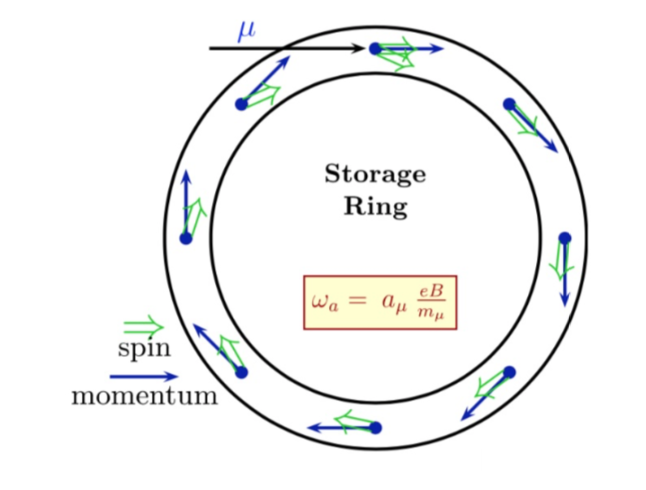
\includegraphics[scale=0.9]{Figures/spin_mom_diff}
\decoRule
\caption{A diagram of how the spin precession direction changes compared to the momentum vector direction whilst travelling through the g-2 storage ring.}
\label{fig:spin_mom_diff}
\end{figure}

This equation depends on $a_\mu$ rather than the magnetic moment and thus $a_\mu$ can be determined directly by the measurement of $\omega_{a}$. The magnetic field B is the only unknown value in this equation. This is required to be known to the same precision as the $\omega_{a}$ and will be discussed in chapter 4.

\section{Relativistic effect on $\omega_{a}$}

At the relativistic energies used by the experiment, an extra effect to the spin frequency occurs called Thomas precession \cite{Chap2Ref2}, which takes into account that the muon is in a rotating reference frame and not an inertial frame. The spin frequency is altered to give
\begin{equation}
\omega_{s} = g\frac{eB}{2m}+(1-\gamma)\frac{eB}{\gamma{m}},
\end{equation}
where $\gamma$ is the Lorentz factor.
Relativistic effects also lead the cyclotron frequency to be 

\begin{equation}
\omega_{c} = \frac{eB}{\gamma{m}}.
\end{equation}

The equation for $\omega_{a}$ is subsequently changed to

\begin{equation}
\omega_{a} = g\frac{eB}{2m}+(1-\gamma)\frac{eB}{\gamma{m}}. -\frac{eB}{\gamma{m}}.
\end{equation}

The relativistic alterations for this equation cancel out to give 
\begin{equation}
\omega_{a} = g\frac{eB}{2m}-\frac{eB}{m} = \bigg(\frac{g}{2}-1\bigg)\frac{eB}{m}.
\end{equation}

\section{Electric field effect on $\omega_{a}$}

The value of $\omega_{a}$ is effected by the electric field from electrostatic quadrupoles, along with instances where the stored muon momentum vectors are not orthogonal to the magnetic field. This leads to changes to the relativistic equations for both $\omega_{s}$ and $\omega_{c}$ that have been previously quoted equations 3.1 and 3.2.

\begin{equation}
\omega_{a} = \frac{e}{m}\bigg[ a_{\mu}B - \bigg(a_{\mu} - \frac{1}{\gamma^2{-1}} \bigg)\frac{\beta{\times}E}{c}-a_{\mu}\bigg(\frac{\gamma}{\gamma+1}\bigg)(\beta\cdot{B})\beta\bigg].
\end{equation}

Instead of using a magnetic field gradient to apply vertical focusing the experiment employs electrostatic quadrupoles to provide the vertical containment of the muon beam. A relativistic particle travelling through the electric field will see a motional magnetic field. However this effect can be cancelled out by choosing muons with a "magic" gamma factor of $\gamma_{magic} = 29.3$. This corresponds to the so called "magic" momentum of 3.094 GeV/c, which is the target momentum for muons in the storage ring and the orbit radius is designed for muons with this momentum. This choice removes the $\beta{\times{E}}$ term by ensuring $a_{\mu}-(\frac{1}{\gamma^2{-1}}) = 0$ and thus $\omega_{a}$ is no longer effected on the electric field.

There are two assumptions that can be used to simplify equation 3.15. The first assumption is that the muons momentum vector direction is orthogonal to the storage ring magnetic field. This simplifies the equation as it means $\beta{\cdot}B = 0$. However a small correction is required due to the small fraction of muons that are not perpendicular to the magnetic field. This leads to muons possessing a vertical betatron oscillation. A correction is required for this effect on $\omega_{a}$ which is called the pitch correction and is discussed in chapter 7.

The second assumption is the use of the magic momentum value to remove the $\beta{\times}E$ term which originates from the electric field used to vertically focus the muon beam. There is however a small spread in the muons momentum, therefore some do not possess the magic momentum. This leads to an additional correction to $\omega_{a}$ called the E-field correction.

Removing these two effects leads to an $\omega_{a}$ given by

\begin{equation}
\omega_{a} = \frac{e}{m}a_{\mu}B.
\end{equation}

\section{Determining $\omega_{p}$}

The magnetic field measurement is carried out by extracting B-field in terms of the free proton Larmor precession frequency $\omega{_p}$. The goal is to measure $\delta\omega_{p} \leq {70}$ppb which is approximately a factor of 2.5 smaller than E821. The value of $\omega_{p}$ is obtained from measurements of the very precise magnetic field. There are several probes used to measure the magnetic field around the ring. These measure the Larmor frequency of a free proton $\omega_{p}$ while in the storage ring field. There is the trolley system which is able to pass through the muon storage volume and is fitted with Nuclear Magnetic Resonance (NMR) probes to carry out measurements of the magnetic field. When the beam is off, the trolley can travel around the storage ring. These measurements are done every 3-5 days and are combined together to obtain the magnetic field as a function of the position.
There are also 378 fixed NMR probes secured to the top and bottom of the storage ring vacuum chambers. Unlike the trolley they can run when the beam is on as they are placed outside the muon storage region and are used to relate the NMR trolley measurement to a measurements carried out while there is beam. A third system of probes act as a calibration probe system between the trolley measurements and the fixed probes. A magnetic field as a function of position and time is produced by combining the various field measurements \cite{Chap2Ref1}.

The final value needed is $\big \langle \omega_{p} \big \rangle$ which is the average field experienced by the muons. To determine this value the muon distribution M(r,t) and the magnetic field as a function of position and time needs to be integrated over the muon distribution as given by

\begin{equation}
\big \langle {\omega_{p}} \big \rangle = \int M(\vec{r},t) {\omega_{p}}(\vec{r},t) dt dV. 
\end{equation}

\section{$a_{\mu}$ calculation}

An $a_{\mu}$ value will be determined from the muon precession frequency $\omega_{a}$ which is obtained by fitting the time spectrum of the decay positrons and the magnetic field calibrated to the Larmor frequency of a free proton. With each value averaged over its position and time in the storage ring.
\noindent
This leads to a simplified equation
\begin{equation}
a_{\mu} = \frac {\omega_{a}/\omega_{p}}{\lambda_{+}-\omega_{a}/\omega_{p}} = \frac {R}{\lambda_{+} -R}.
\end{equation}
 
where  $\lambda_{+} =  {\mu_{\mu+}}{\mu_{p}} = 3.183 345 137 (85)$ is the muon-to-proton magnetic moment ratio. For the BNL E989 experiment the value of R once the E-field and pitch corrections have been applied is $R_{\mu^{+}}= 0.003 707 204 7(26)$ \cite{Reference13}. The value of $\lambda_{+}$ is determined from the measurement of muonium ($\mu^{+}e^{-} atom)$ hyperfine splitting. The use of $\lambda_{+}$ in the $a_{\mu}$ calculation relies on the assumption of CPT invariance and so assumes 
\begin{equation}
a_{\mu+} = a_{\mu-}.
\end{equation}
\begin{equation}
{\lambda_{+}} = \lambda_{-}.
\end{equation}

Therefore a comparison between $R_{\mu+}$ and $R_{\mu-}$ provides a test for CPT \cite{Reference22}\cite{Reference29}. The new Fermilab experiment is also set up to be able to measure $a_{\mu-}$ and this measurement could potentially be done after the $a_{\mu+}$ measurement is completed.


